
% ==================================================
%	Aufbau
% ==================================================

\section{Aufbau}

Der experimentelle Aufbau des Versuches ist in Abbildung~\ref{fig:aufbau}
dargestellt. Hier befindet sich ein \Cs~Strahler in einem Bleibehälter.
Die davon ausgesendete $\gamma$-Strahlung trifft kolliminiert auf den zu
untersuchenden Würfel. Der Würfel besteht aus den $3\times 3 \times 3$
Elementarwürfeln, wobei jeder Elementarwürfel eine Seitenlänge von \SI{1}{\cm}
hat. Zudem befinden sich die Elementarwürfel in einem Aluminiumwürfel mit einer
Wandstärke von \SI{1}{\mm}. Der Würfel kann zur Einstellung der Strahlrichtung
um die $z$-Achse rotiert werden und senkrecht zur Strahlrichtung verschoben
werden. Nach Durchdringen des Würfels trifft der Strahl auf einen NaJ-Detektor.
Der NaJ-Detektor ist ein Szintillator, welcher aus NaJ dotiert mit
Thallium besteht. In dem Szintillator wird die
$\gamma$-Strahlung durch deren Wechselwirkung mit Materie
(überwiegend innere Photo-Effekt) nachgewiesen.\cite{kern_und_teilchenphysik}
% Der NaJ-Detektor ist ein Szintillator, sodass die $\gamma$-Strahlung durch
% deren Wechselwirkung mit Materie (überwiegend innere Photo-Effekt),
% in diesem Fall NaJ dotiert mit Thallium,
% nachgewiesen wird.\cite{kern_und_teilchenphysik}
Die von den $\gamma$-Quanten deponierte Energie wird in
Licht umgewandelt und anschließend von einem Photomultiplier nachgewiesen.
Die Dotierung des NaJ-Kristalls ist notwendig, um lokal das Leitungsband zu
verformen. Bei dem NaJ-Kristall ist das Valenzband vollständig besetzt und das
Leitungsband leer. Die Bandlücke beträgt dabei ca. \SI{6-8}{\eV}.
Ein $\gamma$-Quant mit $\sim \SI{1000}{\eV}$ ist somit in der Lage ca. 100
Elektronen in das Leitungsband zu heben. Diese angeregten Elektronen fallen
unter Aussendung von Licht mit \SI{6-8}{\eV} wieder in das Valenzband zurück.
Das ausgesandte Licht ist aber nun wieder in der Lage andere Elektronen ins
Leitungsband zu heben, sodass der Kristall für das Licht undurchlässig wäre.
Die Dotierung mit Thallium verringert die Bandlücke lokal, sodass Photonen mit
ca. \SI{3}{\eV} bei Rekombination erzeugt werden können, welche nicht in der
Lage sind neue Elektronen anzuregen und den Kristall verlassen können.
Die niederenergetischen Photon gelangen zum Photomultiplier, wo sie durch den
äußeren Photo-Effekt Elektronen aus einer Photokathode mit entsprechender
Austrittsarbeit lösen. Diese Elektronen werden durch eine Kaskadenschaltung von
Dynoden beschleunigt und vervielfacht, sodass am Ende eine messbare von
Rauschen zu unterscheidende Spannung abgegriffen werden kann.
Diese Spannungspulse werden letztendlich von einem Multichannelanalyzer
analysiert und am Computer von einem Hilfsprogramm in einem Histogramm
aufsummiert.

\begin{figure}[htpb]
  \centering
  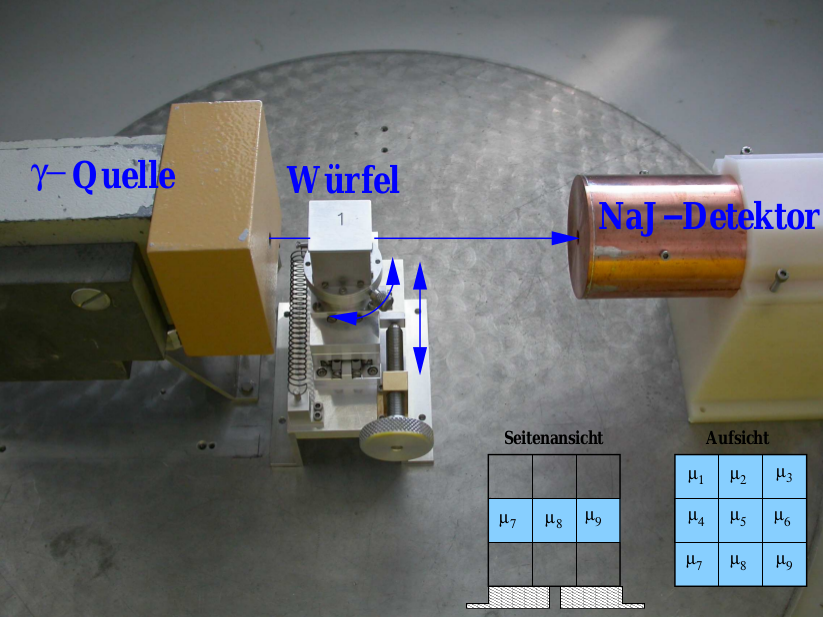
\includegraphics[scale=0.3]{bilder/aufbau.png}
  \caption{Experimenteller Aufbau.\cite{AP}}
\label{fig:aufbau}
\end{figure}
